\chapter{Implementation}
\label{cha:implementation}

The previous chapter described the design of the product. During the
implementation, issues with the design surface that have not been foreseen in
advance. This chapter discusses these issues and the changes made to the design
to resolve them. \Cref{sec:dynsem-eval-strat} discusses the implementation
of the evaluation strategy for DynSem. \Cref{sec:esv-extensions} explains the
extensions that have been made to Spoofax's Editor Services to enable the
language designer to configure and extend the REPL for their
language. \Cref{sec:injection} discusses the use of dependency injection via the
Guice framework.  \Cref{sec:frontends} discusses the implementation of the
console and Eclipse frontends.

\section{DynSem Evaluation Strategy}
\label{sec:dynsem-eval-strat}
An implementation for the \texttt{IEvaluationStrategy} as discussed in
\cref{sec:eval-strat} has been made for languages that specify their dynamic
semantics using DynSem. The implementation class, called
\texttt{``DynSemEvaluationStrategy''} (see \cref{fig:uml-dynsem-eval-strat}),
evaluates REPL-specific DynSem rules and maintains the environment in which
evaluation takes place.

This section first goes over the configuration interface for DynSem that is
provided by the REPL. After that, the implementation of DynSem and of the
\texttt{DynSemEvaluationStrategy} are discussed in more detail.

\subsection{The REPL configuration interface}
\label{sec:impl-repl-spec}
To evaluate a program in their language within the REPL, the language designer
has to make two kinds of configurations for the REPL in their DynSem
specification. The first is a rule for initializing the execution environment
for the REPL, shown in \cref{lst:shell-init}. The second are the rules for
implementing the REPL-specific semantics as discussed in
\cref{ssec:repl-spec-semant}.

\paragraph{Environment initialization} The initialization rule shown in
\cref{lst:shell-init} is evaluated upon the initialization of the evaluation
strategy. It instantiates the semantic components that form the execution
environment for the REPL: an environment with an initial variable binding of
$x \mapsto 4$, and an empty store. The evaluation strategy uses this in its
successive evaluations, and updates the execution environment after each result.

\begin{minipage}{\textwidth}
\begin{lstlisting}[language=dynsem,caption={The initialization rule for the
semantic components.},label={lst:shell-init},numbers=left]
rules
  // Initialization of shell state: an environment with "x" bound to 4,
  // and an empty store.
  ShellInit() -init-> ShellInit() :: Env { "x" |--> NumV(4) }, Store {}.
\end{lstlisting}
\end{minipage}

\paragraph{REPL-specific semantics} The second kind of configuration are the
rules for the REPL-specific semantics. These can be seen as entry points for the
REPL to the interpreter. The rules are all named ``shell'', so that they are
distinct of the ordinary semantics. \Cref{lst:shell-rule} shows an example of
such a rule. The rule implements a construct that is only valid when evaluating
within the REPL: it implements binding the result of an expression to a
variable. With the specification of this rule, the bound variable can be used in
successive evaluations done by the user.

Note that the environment \textit{E} is passed as a read-write component,
instead of a read-only component as is explained in \cref{ssec:dynsem}. This is
because in this case the environment \emph{should} be writable, since the
resulting environment after execution should be available to the REPL. Note also
that in line 5 of the rule, the rest of the specification is recursively
invoked. This shows that much of the existing specification can be reused when
implementing the REPL-specific semantics.

\begin{minipage}{\textwidth}
\begin{lstlisting}[language=dynsem,caption={A rule specifying semantics specific
to the REPL.},label={lst:shell-rule},numbers=left]
rules
  // let x = 2
  Let(x, e) :: E -shell-> v :: E'
  where
    E |- e :: Store {} --> v :: Store _;
    E |- bindVar(x, v) --> E'.
\end{lstlisting}
\end{minipage}

\subsection{The implementation}
\label{ssec:implementation}
This subsection discusses the implementation of the evaluation
strategy. However, before doing this, an explanation of the interfaces provided
by DynSem and its generated interpreters is in order.

\paragraph{DynSem's generated interpreters} As explained in \cref{ssec:dynsem},
DynSem is able to generate interpreters in Java from a dynamic semantics
specification written in the DynSem meta-language. DynSem uses the Truffle
language implementation framework for its generated
interpreters~\cite{Humer14}. By using the Truffle framework, the generated
interpreter can benefit from the performance optimizations of the Truffle
virtual machine (VM)~\cite{Wurthinger13}, as opposed to writing ones own
optimizations instead.

The evaluation of a program is done by invoking a reduction rule with as its
arguments the program in the form of an AST, and the semantic components. A
reduction rule can be found by performing a lookup with the rule's signature as
the lookup key, through Truffle's foreign object access
interface~\cite{Grimmer15}. That is, the foreign objects are precisely the rules
such as the one shown in \cref{lst:shell-rule} (in the form of an internal
representation).

For this reason, the interpreter generated by DynSem can be seen as a
\textit{meta-interpreter}: it interprets a DynSem specification, and allows
access to rules as value objects through Truffle's foreign object access
interface. The rules themselves (or the ``values'' interpreted by the
meta-interpreter) can then be seen as access points to the interpreter of the
language, as they can be invoked with an AST and semantic components. The
relation between a meta-interpreter and an ordinary interpreter is captured in
the diagram shown in \cref{fig:meta-interpreter}.

\begin{figure}[b]
  \centering
  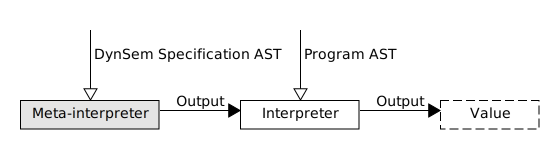
\includegraphics[width=0.8\textwidth]{meta-interpreter}
  \caption{The relation between a meta-interpreter and an ordinary interpreter.}
  \label{fig:meta-interpreter}
\end{figure}

\paragraph{The implementation of the evaluation strategy} The UML diagram of the
evaluation strategy is shown in \cref{fig:uml-dynsem-eval-strat}. The
\texttt{DynSemEvaluationStrategy} uses an \texttt{``IInterpreterLoader''} to
load the interpreter as generated by DynSem. It initializes the Truffle VM,
called the \texttt{``PolyglotEngine''}, with the interpreter generated by
DynSem, by evaluating the DynSem specification through the \texttt{eval} method
provided by the \texttt{PolyglotEngine}.

The \texttt{PolyglotEngine} furthermore provides the \texttt{findGlobalSymbol}
method, allowing the evaluation strategy to lookup the reduction rules of the
interpreter represented as a \texttt{``Value''} object. The returned
\texttt{Value} object has an \texttt{execute} method, which provides the
interface for invoking the reduction rule with the program AST and the semantic
components. This way, the configuration interface as outlined in
\cref{sec:impl-repl-spec} can be implemented: the initialization rule and the
REPL-specific rules can simply be looked up by their rule signature.

\begin{figure}[t]
  \centering
  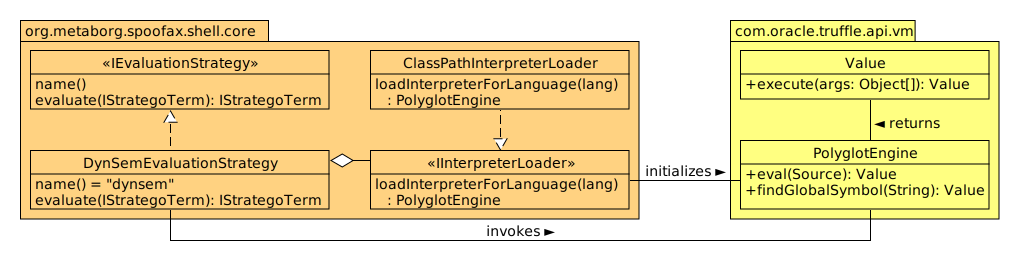
\includegraphics[width=\textwidth]{uml-dynsem-eval-strat}
  \caption{UML diagram of the \texttt{DynSemEvaluationStrategy} and its
    collaborator \texttt{IInterpreterLoader}.}
  \label{fig:uml-dynsem-eval-strat}
\end{figure}

%%% Local Variables:
%%% mode: latex
%%% TeX-master: "../main"
%%% End:


\section{Dependency Injection}
\label{sec:injection}

The design of Spoofax relies quite heavily on dependency injection by the Guice
framework.  To achieve as much interopability as possible, the final product
uses dependency injection in the same spirit as Spoofax. Guice has had a
substantial impact on the design and implementation of the final product, since
Guice nearly eliminates the need to create factories for complex datatypes.

Guice requires the programmer to bind implementations of dependencies in its
module classes, thereby separating behavior and dependency resolution.  Complex
datatypes can then accept their dependencies as constructor arguments, allowing
Guice to resolve and inject an instance of a bound type.

In the final product dependency injection is also used to supply several classes
with a default configuration.  An example is the default list of commands
available to a user as described in \cref{sec:commands}.  The list of commands
is created from a Guice module by instantiating a \texttt{MapBinder} with
predefined bound commands. Child modules can then append extra entries to the
\texttt{MapBinder}, which makes them directly available to the existing
architecture.

Using dependency injection has made it easier to create a modular product,
mostly centered around smaller interfaces interacting with each other. All these
interfaces can easily be bound to new implementations, thereby extending the
functionality of the REPL.


\section{Frontends}
\label{sec:frontends}

\Cref{cha:design} showed that the backend places few restrictions on the
frontends. A good example of this fact is the visitor pattern (see
\cref{sec:visitor}), which allows the frontends to schedule the processing of
the results and to display them in many different ways.  To illustrate this
flexibility, two frontends have been developed: a single threaded, text-based
console frontend and a multithreaded, graphical plugin to the Eclipse IDE. Both of these
are discussed next.

\subsection{Console frontend}
\label{ssec:consolerepl}

The console frontend provides the user with a text-based user interface. For users
already accustomed to the command line, this is perhaps the most familiar
looking interface, see \cref{fig:frontend-console}.

\begin{figure}[h]
  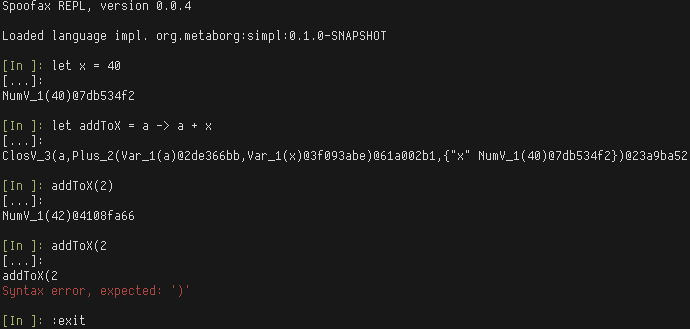
\includegraphics[width=\textwidth]{console-frontend}
  \caption{The console frontend.}
  \label{fig:frontend-console}
\end{figure}

A REPL running in the console requires a means of getting
user input from the standard input stream and printing results and error
messages to the standard output and error streams.

A BSD-licensed library that features these requirements is JLine2.
JLine2 is a library for handling console input, similar to GNU readline and BSD
editline. Most of the editing features present in these two libraries are also
present in JLine2.

\begin{figure}[h]
  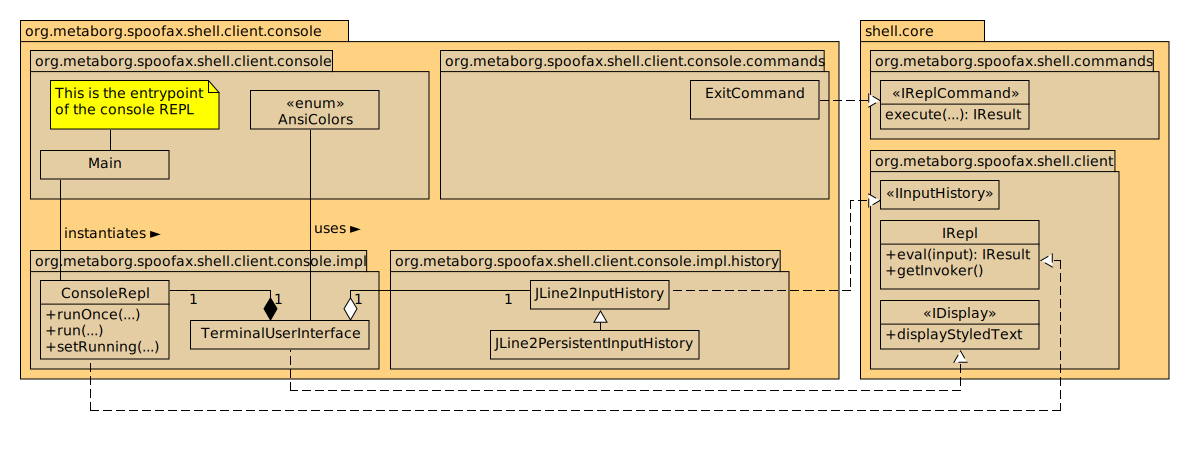
\includegraphics[width=\textwidth]{uml-console}
  \caption{UML diagram for the console frontend.}
  \label{fig:uml-console}
\end{figure}

As can be seen in \cref{fig:uml-console}, a frontend has to implement only a few
interfaces. The \texttt{ConsoleRepl} class is the central element in the
console frontend. It is instantiated first and controls the lifecycle of this
frontend. Its \texttt{run} method maps to the \texttt{loop} step in
Read-Eval-Print Loop and thus contains the \texttt{read}, \texttt{eval} and
\texttt{print} steps.

The \texttt{read} and \texttt{print} steps are provided
the by \texttt{TerminalUserInterface} class, which, as the name implies, is
responsible for the user interface. This class has connections to the standard
input, output and error streams. It uses JLine2 to provide a blocking input
editor. Because the input editor is blocking, the console frontend can run in a
single thread, thereby greatly simplifying its implementation.

A straightforward algorithm to provide multiline editing capabilities is used in
combination with JLine2's input buffer.
JLine2 does support input history, which means only an adapter class,
\texttt{JLine2InputHistory}, had to be made to interoperate with the history
interface that is offered by the backend. An extension to this class is provided
to maintain persistent history.

To provide syntax and error highlighting, ANSI color codes are used. These
color codes are obtained through the \texttt{AnsiColors} enumeration, which
maps colors as returned by the \texttt{IResult} interface to their closest
ANSI equivalent.

Lastly, an \texttt{ExitCommand} is provided to halt the \texttt{run} method
in \texttt{ConsoleRepl}.

\subsection{Eclipse plugin}
\label{ssec:eclipse-plugin}

Spoofax currently features extensive integration in the Eclipse IDE. The client
expressed their interest to have this same level of integration for the REPL. A
plugin to the Eclipse IDE has been developed, which exposes the REPL
functionality through a graphical user interface that is familiar to anyone
working in Eclipse, see \cref{fig:frontend-eclipse}.

\begin{figure}[h]
  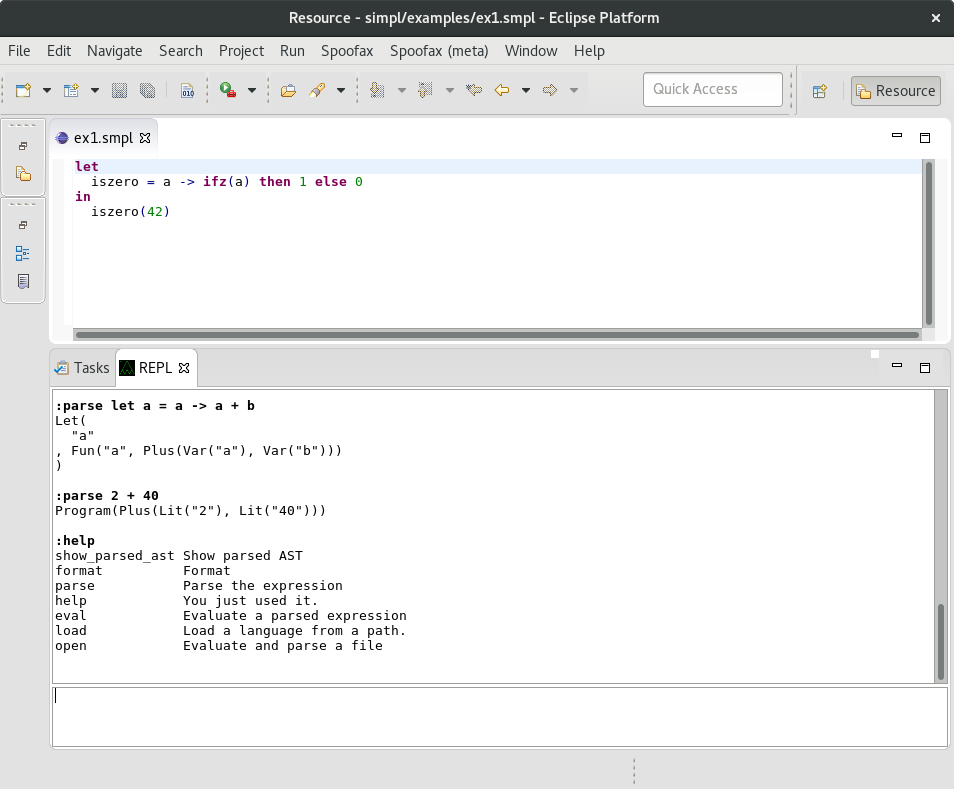
\includegraphics[width=\textwidth]{frontend-eclipse}
  \caption{The Eclipse plugin.}
  \label{fig:frontend-eclipse}
\end{figure}

As is customary for a graphical user interface toolkit, the toolkit offered by
Eclipse uses multiple threads. One such thread is designated the ``UI thread'',
or user interface thread. This thread is responsible for processing
user-generated events (such as mouse clicks) and updating the graphical
representation of the widgets. All tasks that perform long running
calculations are supposed to be run in a background thread, such that the UI
thread is free to process incoming events. Instead, if a long running
computation is run in the UI thread, the widgets on the screen stop responding
to the user and the program appears to be in a frozen state. For this reason,
the backend has to perform its evaluations in a background thread, whilst all
the widgets and user interaction takes place in the UI thread.
The following discussion refers to the UML as depicted in
\cref{fig:uml-eclipse}.

\begin{figure}[b]
  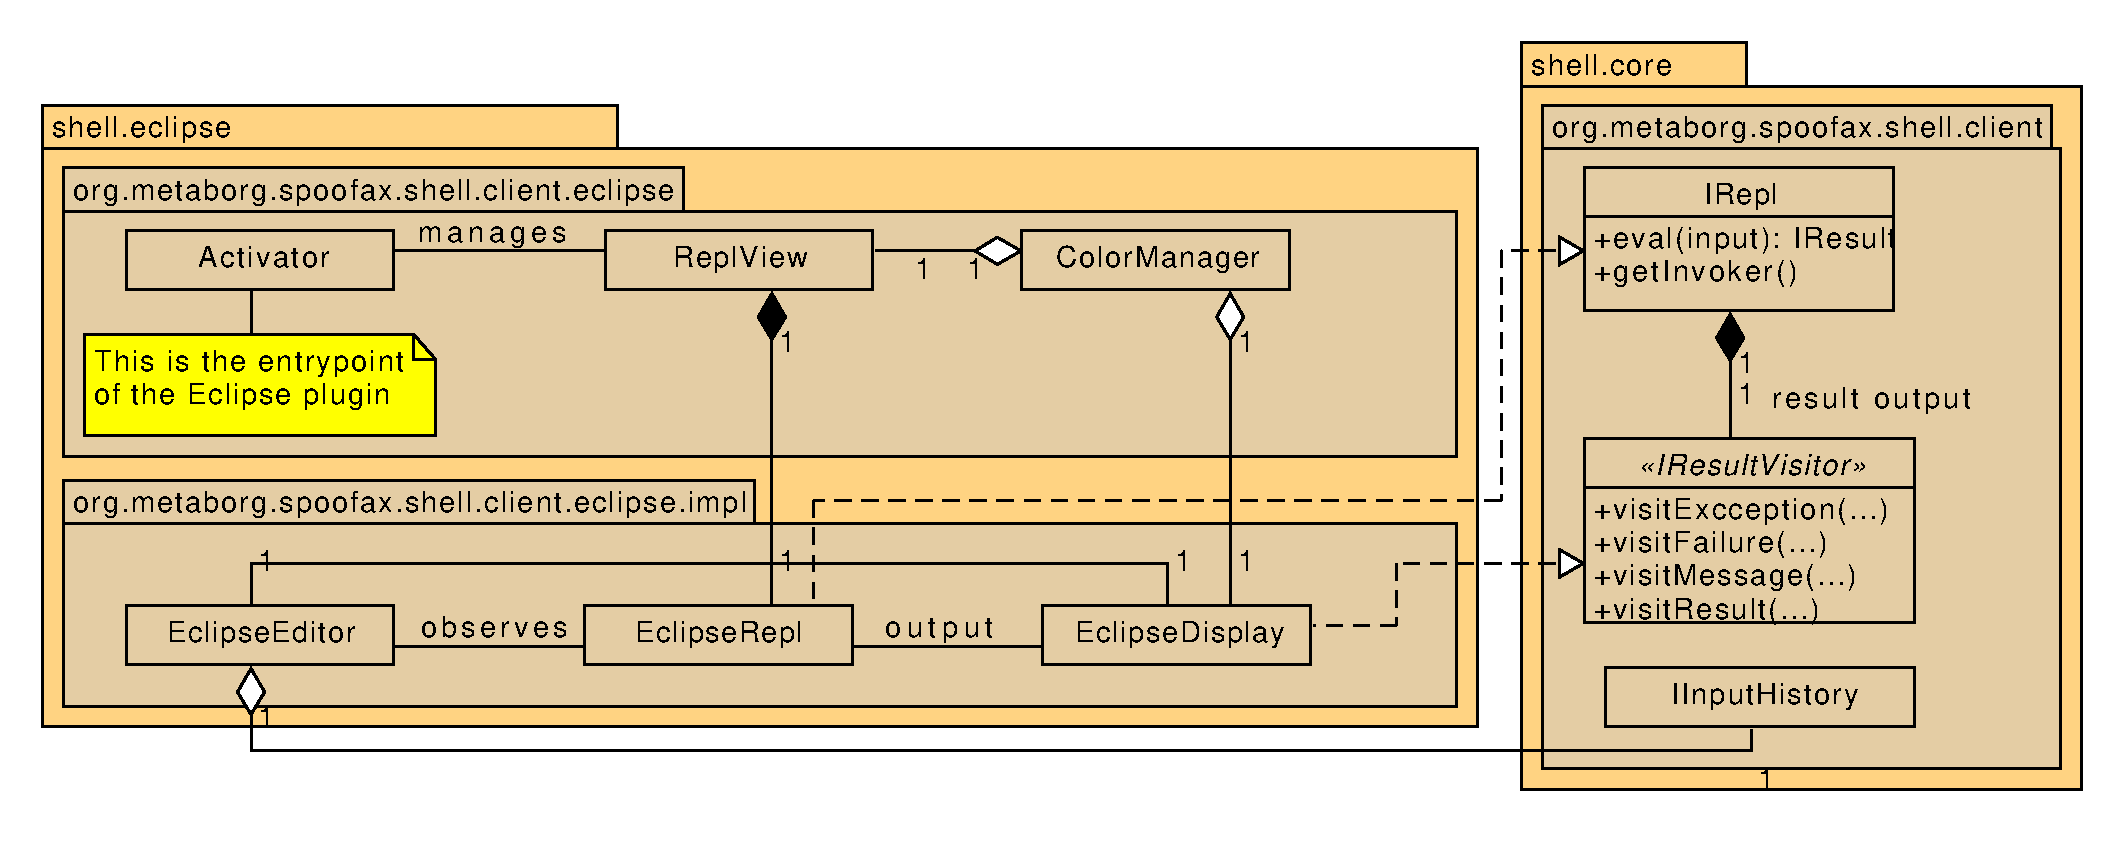
\includegraphics[width=\textwidth]{uml-eclipse}
  \caption{UML diagram for the Eclipse plugin.}
  \label{fig:uml-eclipse}
\end{figure}

Again, as can be seen in the UML, only a few interfaces have to be implemented.
The \texttt{EclipseRepl} class is the central element in the Eclipse plugin.
It is instantiated by the \texttt{ReplView} class, which in turn is
instantiated by Eclipse when the user requests the REPL to be opened. This
\texttt{ReplView} class also instantiates the input editor widget,
\texttt{EclipseEditor} and the \texttt{IDisplay} implementation,
\texttt{EclipseDisplay}.
In a multithreaded graphical user interface environment, asking text entry
widgets for the entered text is rarely a blocking process. This is no different
in Eclipse. For this reason, the \texttt{EclipseRepl} cannot simply loop as the
console frontend does. The solution is to use reactive programming through RxJava:
the \texttt{EclipseRepl} is registered as an observer to the
\texttt{EclipseEditor}. When the user presses the Return key,
\texttt{EclipseEditor} notifies \texttt{EclipseRepl} with the contents of its
text buffer. \texttt{EclipseRepl} in turn launches a background job in which the
evaluation takes place, so as to not block the UI thread. Since the backend
simply returns an implementation of the \texttt{IResult} interface (see
\cref{sec:visitor}), the \texttt{EclipseRepl} can schedule the processing of this
result by the \texttt{EclipseDisplay} class on the UI thread. This processing
has to be done on the UI thread, because otherwise the \texttt{EclipseDisplay}
cannot update the widget it maintains to display results.
As one can see, the Eclipse plugin does not implement the \texttt{loop} step of
a REPL. There is no need to do so, due to the use of multithreading and reactive
programming.

%%% Local Variables:
%%% mode: latex
%%% TeX-master: "../main"
%%% End:


%%% Local Variables:
%%% mode: latex
%%% TeX-master: "main"
%%% End:
